\documentclass[12pt]{extarticle}
\usepackage{tempora}
\usepackage[T1, T2A]{fontenc}
\usepackage[utf8]{inputenc}
\usepackage[english, ukrainian]{babel}
\usepackage{geometry}
\usepackage{graphicx}
\usepackage{multirow}
\usepackage{multicol}
\usepackage{float}
\graphicspath{{/home/artem/Pictures}}
\geometry
{
    a4paper,
    left=30mm,
    top=15mm,
    right=20mm,
    bottom=15mm,
}

\begin{document}
\begin{titlepage}
    \begin{center}
        \textbf{\normalsize{\MakeUppercase{
            Міністерство Освіти і науки України
            Національний університет "Львівська політехніка"
        }}}

        \begin{flushright}
        \textbf{ІКНІ}\\
        Кафедра \textbf{ПЗ}
        \end{flushright}
        \vspace{15mm}

        \includegraphics[width=0.4\textwidth]{lpnu_logo.png}

        \vspace*{\fill}

        \textbf{\normalsize{\MakeUppercase{Звіт}}}
            
        До лабораторної роботи №10

        \textbf{на тему:} “Метод пошуку Кнута-Мориса-Прата”

        \textbf{з дисципліни:} "Алгоритми і структури даних”
            
        \vspace*{\fill}

        \begin{flushright}

            \textbf{Лектор:}\\
            доцент кафедри ПЗ\\
            Коротєєва Т. О.\\
            \vspace{12pt}

            \textbf{Виконав:}\\
            студент групи ПЗ-24\\
            Губик А. С.\\
            \vspace{12pt}

            \textbf{Прийняв:}\\
            асистент кафедри ПЗ\\
            Вишневський К. О.\\
        \vspace{12pt}
        \end{flushright}

        Львів -- 2023
            
            
    \end{center}
\end{titlepage}

\subsection*{Тема роботи} 
Метод пошуку Кнута-Мориса-Прата.

\subsection*{Мета роботи} Вивчити алгоритм пошуку Кнута-Мориса-Прата. Здійснити програмну реалізацію алгоритму пошуку Кнута-Мориса-Прата. 
\subsection*{Індивідуальне завдання}
У файлі задано дві стрічки S та P. Довжина стрічок більша 0 і менша 10000, стрічки містять лише букви латинського алфавіту. Вивести номери символів в  порядку спадання починаючи з яких стрічка P входить в стрічку S.
\subsection*{Індивідуальне завдання}

\begin{enumerate}
    
\item Для заданого слова визначити префікс-функцію D

\item Встановити і=0, j=0, d=1.

\item Поки j<m, i<n

\item Перевірка: якщо S[i]=P[j], то d++, i++.j++ поки d != m.

\item Якщо j == n-1 повернути i-j, інакше овернути -1
\item  

\item Кінець.
\end{enumerate}
\subsection*{Теоретичні відомості}
На вхід поступають два масиви символів - S розміром n (текст) та P розміром m (слово). Необхідно знайти перше входження слова в тексті. Схема алгоритму полягає у поступовому порівнянні слова з текстом та у разі знайденого неспівпадіння зробити зсув по тексту на крок, що дорівнює різниці кількості співпавших символів та значення відповідної префікс-функції. Алгоритм використовує просте спостереження, що коли відбувається неспівпадіння тексту і слова, то слово містить у собі достатньо інформації для того, щоб визначити, де наступне входження може початися, таким чином пропускаючи кількаразову перевірку попередньо порівняних символів. Попередньо проводиться дослідження слова та визначається префікс-функція.

Префікс-функція стрічки– це довжина найбільшого префікса стрічки S[1..i], який не співпадає з цією стрічкою і одночасно є її суфіксом. Простіше кажучи, це довжина найбільшого  початку стрічки, що одночасно є її кінцем.
\subsection*{Вихідний код}

{\fontfamily{pcr}\selectfont
\begin{verbatim}
    #include <iostream>
    #include <fstream>
    #include <vector>
    #include <string>
    
    std::vector<int> computeLPS(const std::string& pattern) {
        int patternLength = pattern.length();
        std::vector<int> lps(patternLength, 0);
        int j = 0; // Length of the previous longest prefix suffix
    
        for (int i = 1; i < patternLength; ++i) {
            while (j > 0 && pattern[i] != pattern[j]) {
                j = lps[j - 1];
            }
    
            if (pattern[i] == pattern[j]) {
                lps[i] = ++j;
            }
        }
        return lps;
    }
    
    int findFirstOccurrence(const std::string& text, const std::string& pattern) {
        int textLength = text.length();
        int patternLength = pattern.length();
        std::vector<int> lps = computeLPS(pattern);
        for(int i : lps)
            std::cout << i << ' ';
        std::cout << std::endl;
        int j = 0; // Index for pattern[]
    
        for (int i = 0; i < textLength; ++i) {
            while (j > 0 && text[i] != pattern[j]) {
                j = lps[j - 1];
            }
    
            if (text[i] == pattern[j]) {
                if (j == patternLength - 1) {
                    return i - j; // Return the start index of the first occurrence
                } else {
                    j++;
                }
            }
        }
        return -1; // Pattern not found in text
    }
    
    int main() {
        std::ifstream file("input.txt"); // Replace "input.txt" with your file name
        if (!file.is_open()) {
            std::cout << "Unable to open file!" << std::endl;
            return 1;
        }
    
        std::string S, P;
        if (std::getline(file, S) && std::getline(file, P)) {
            int index = findFirstOccurrence(S, P);
            if (index != -1) {
                std::cout << "Pattern P found at index: " << index << std::endl;
            } else {
                std::cout << "Pattern P not found in string S" << std::endl;
            }
        } else {
            std::cout << "File does not contain both strings!" << std::endl;
        }
    
        file.close();
        return 0;
    }
    
\end{verbatim}
}
\vspace{12pt}
\begin{figure}[H]
    \centering
    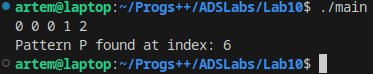
\includegraphics[width=0.90\textwidth]{Screenshot_20231129_090230}
    \caption{}
\end{figure}

\subsection*{Висновок} 

Я ознайомився з алгоритмом Кнута-Моріса-Прата і що таке Longest Suffix Prefix.

\end{document}
